\chapter{Palabras acumuladas}
% Intro {{{

La búsqueda para cuantificar la influencia, ha llevado a contar las
palabras que son nuevas en los distintos receptores, para después asociarlas con  campos semánticos y sucesos históricos que respalden su aparición. Sin embargo, el proceso anterior, sólo brinda información del año en que migraron las palabras, no se sabe lo que pasa con ellas en los años posteriores a su migración. 

Antes de seguir con el desarrollo de este capítulo, conviene definir como \textbf{préstamos acumulados} a aquellas palabras con origen \textit{A} que ya habían aparecido en \textit{B}, y para un determinado año lo vuelven a hacer.  La diferencia entre los préstamos nuevos y los préstamos acumulados, es que solo serán nuevos en el año de aparición, posteriormente se convertirán en acumulados.

Los préstamos acumulados serán útiles para obtener una cantidad medible con la cual interpreta la influencia y con ella saber que sucede con las palabras migrantes después del primer año de aparición.  Para lograr tal cantidad, se realizaron los siguientes pasos.



\begin{enumerate}
	\label{proceso_uso}
	
	\item  Dada la lista de las cinco mil palabras mas usadas de \textit{B} en el año $t$, se obtiene la \textbf{frecuencia total} $\underset{\text{\tiny B}}{F}(t)$ al sumar las frecuencias $f(k)$ de todas las palabras en la lista, donde $k$ determina el rango  de cada palabra.
	
	\begin{equation}
	\label{ec.ftot}
	%F^{y}_{\text{B}} = \sum_{k=1}^{5000} f(k)
	\underset{\text{\tiny B}}{F}(t) = \sum_{k=1}^{5000} f(k)
	\end{equation}

	
	\item Si se distinguen los préstamos acumulados con origen \textit{A}  que tienen rango $j$,  se procede a sumar la frecuencia $f(j)$ de estas palabras.  Esta cantidad será la  \textbf{frecuencia de préstamo} $\underset{ \text{\tiny A} \to  \text{\tiny B} }{P}(t)$   de \textit{A} en \textit{B} para el año $t$.
	
	\begin{equation}
	\label{ec.fpres}
	%P^{y}_{\text{A} \to \text{B}} = \sum_{j} f(j)
	\underset{ \text{\tiny A} \to  \text{\tiny B} }{P}(t) = \sum_{j} f(j)
	\end{equation}
	
	
	\item Si se normaliza la frecuencia de préstamo al dividirla entre la frecuencia total, se obtiene el \textbf{uso} $\underset{ \text{\tiny A} \to  \text{\tiny B} }{U}(t)$  de \textit{A} en \textit{B}.  Esta será la cantidad  que cuantifique la influencia de \textit{A} en \textit{B}.
	
	\begin{equation}
	\label{ec.fuso}
	\underset{ \text{\tiny A} \to  \text{\tiny B} }{U}(t) = \frac{	\underset{ \text{\tiny A} \to  \text{\tiny B} }{P}(t)}{\underset{\text{\tiny B}}{F}(t) }
	\end{equation}
	 
	%\item Se empleó la ecuación \ref{ec.fuso} en todos los años del conjunto de búsqueda, obteniendo 109 valores.
	
	%\item El proceso se repitió para todas las combinaciones de orígenes y receptores.
	
\end{enumerate}

Si en una lista de las palabras más usadas del idioma \textit{B}, se encuentran préstamos acumulados con diferentes orígenes \textit{A}, \textit{C} o \textit{D}. Cada origen tendrá un valor correspondiente de uso. Si se obtienen diferentes valores del uso a lo largo del tiempo,  con ellos se puede estimar cual origen es más utilizado en \textit{B},  en consecuencia cual de ellos tiene una mayor influencia en \textit{B}.

Como en el uso intervienen los préstamos acumulados, se podrá decir cuales son las palabras migrantes que modifican el uso de un idioma en otro. Por ejemplo, si el uso aumenta en un periodo de tiempo $\Delta t$,  las palabras que más descendieron en rango $k$ durante el mismo periodo,  son las causantes del aumento. 


\section {El uso entre idiomas} 

Antes de calcular el uso entre idiomas, se obtuvieron los préstamos nuevos de \textit{A} en \textit{B} durante los años del conjunto base (1740-1899).
Estas palabras servirán como una base para calcular el uso de \textit{A} en \textit{B} dentro de los años del conjunto de búsqueda (1900-2009), ya que si alguna de ellas aparece en una determinada lista de \textit{B}, será un préstamo acumulado. 

Los préstamos nuevos encontrados en el capítulo anterior, servirán como complemento, ya que también seŕan candidatos a ser prestamos acumulados.

Se agruparon los préstamos acumulados por cada pareja de idioma origen e idioma receptor, y por cada año en el conjunto de búsqueda  Se proporciona en \cite{prestamos_acumulados} las listas con las agrupaciones realizadas, mientras que en \ref{lectura.listas} se especifica la forma de leerlas e interpretarlas. Estas listas serán útiles para los siguientes capítulos. 

Al igual que en los préstamos nuevos, existen tres formas de resultados,  la primera es al fijar un origen,  y lograr el uso que este tiene en los demás; en la segunda se obtiene el uso que los demás idiomas tienen sobre un receptor fijo;  mientras que en la tercera se consigue el uso entre dos idiomas. 

%Por cada idioma se presentan dos graficas, la primera al fijar un origen para observar el uso que tiene en los demás; la segunda es el caso contrario,  al graficar el uso de los demás en el.  Una tercera grafica es posible, al representar unicamente el uso entre dos idiomas, estas graficas se agregaran en la sección \ref{palabras.acumuladas.apendice} del Apéndice A.

Para complementar los resultados del capitulo anterior, se expondrán las palabras que intervienen en las épocas donde el uso se vea alterado, sólo se mencionaran aquellas que compartan el mismo campo semántico. 

Adicionalmente, la tabla \ref{tab.cantidad_acumulados} muestra la cantidad promedio de préstamos acumulados, encontrados en el conjunto de búsqueda. La idea  entre la tabla y del uso, es notar que el idioma que más préstamos acumulados tiene en  un receptor no es siempre el de mayor uso.  El uso es mayor si los préstamos tienen rangos mas bajos (frecuencias altas), sin importar cuantos sean. 


\begin{table}
	\centering
	\begin{tabular}{lcccccc}
		\multicolumn{7}{c}{R E C E P T O R}                                                                                                                                             \\
		\multirow{6}{*}{\begin{tabular}[c]{@{}l@{}}O\\ R\\ \,I\\ G\\ E\\ N\end{tabular}} &             & \textbf{inglés} & \textbf{francés} & \textbf{alemán} & \textbf{italiano} & \textbf{español} \\
		& \textbf{inglés} & -           & 324.43      & 164.33      & 77.5        & 73.61       \\
		& \textbf{francés} & 297.36      & -           & 94.06       & 118.55      & 66.31       \\
		& \textbf{alemán} & 63.87       & 48.06       & -           & 34.92       & 16.61       \\
		& \textbf{italiano} & 77.82       & 100.62      & 47.9        & -           & 219.45      \\
		& \textbf{español} & 118.43      & 84.22       & 29.85       & 311.97      & -          
	\end{tabular}
	\caption{Cantidad promedio por año de préstamos acumulados entre idiomas. Se aprecian dos relaciones reciprocas entre el inglés con el francés y el español con el italiano, donde no importa cual actué como receptor, el otro idioma es el origen del que provienen la mayor cantidad de palabras.}
	\label{tab.cantidad_acumulados}
\end{table}




\subsection{Inglés} % {{{

\begin{figure}[h!]
	\centering
	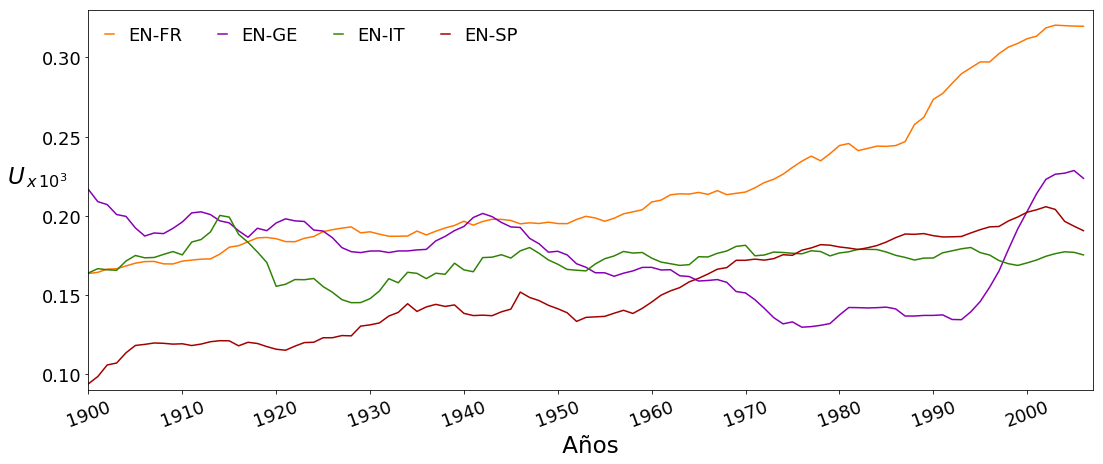
\includegraphics[scale=.38]{UO_EN.png}
	\caption{El uso del inglés en los demás idiomas. El alemán es el idioma donde el uso del inglés ha aumentado más rápido, a razón de  0.05 por cada año desde 1990. También en el alemán el uso del inglés decayó más rápido a razón de 0.0013 por cada año entre 1940 y 1980.}
	\label{fig.UO_EN}
\end{figure} 


De la figura~\ref{fig.UO_EN} se puede ver que el uso del inglés en el francés, en el español y en el italiano aumentó después de 1940, mientras que en el alemán fue posterior a 1990.  La razón de estos aumentos, se asocia con el surgimiento de los Estados Unidos como una potencia mundial después de finalizar la Segunda Guerra Mundial,  al  imponer  su modelo económico e impulsar el desarrollo de la ciencia y la tecnología durante la Guerra Fría.

Los préstamos acumulados  que son comunes en los cuatro receptores, son referentes a los campos semánticos de la economía y de la tecnología. Entre ellos \textit{capital}, \textit{dollar}, \textit{invesment}, \textit{relations}, \textit{market}, \textit{company}, \textit{development}, \textit{financial},  \textit{institutions}, \textit{internet}, \textit{windows} y \textit{software}. 

Otros préstamos son los apellidos de los presidentes de los Estados Unidos (posteriores a la guerra), todos fueron relevantes durante el periodo en el cual gobernaron. 


\begin{figure}[h!]
	\centering
	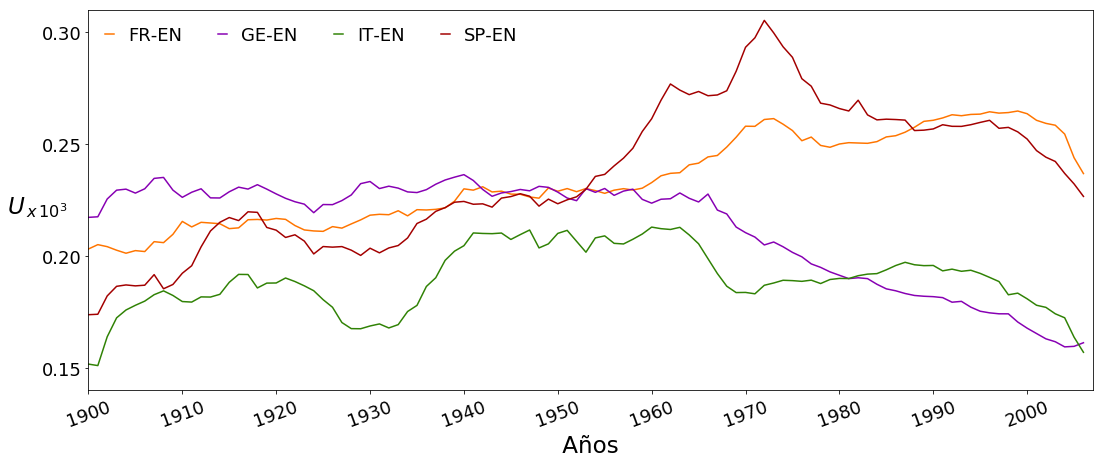
\includegraphics[scale=.38]{UR_EN.png}
	\caption{El uso de los demás idiomas en el inglés. El español y el francés son los idiomas más utilizados en el inglés, aumentando su 
	En los últimos 50 años, el español y el francés han sido los idiomas más utilizados. Tras la segunda guerra mundial, alemán e italiano decayeron consistente en ser lenguas de los países vencidos.}
	\label{fig.UR_EN}
\end{figure} 


De la figura~\ref{fig.UR_EN} se puede ver que entre 1940 y 1960, el uso de los demás idiomas en el inglés era similar, alrededor de 0.21 $\pm$ 0.01. Después de finalizar la Segunda Guerra Mundial, el uso del alemán y del italiano en el inglés decayó,  consecuencia de que Alemania e Italia perdieran la guerra.

Por otra parte tanto el español como el francés aumentaron su uso en el inglés después de la Segunda Guerra Mundial. Referente al francés, los préstamos acumulados más comunes son del campo semántico de la religión,, por ejemplo \textit{dieu}, \textit{eveque}, \textit{religion}, \textit{saint} y \textit{eglise}.

Con el español, los préstamos continuamente utilizados son nombres de países latinoamericanos. Con alguno de ellos los Estados Unidos tuvieron una relacio histórica como \textit{mexico} y \textit{cuba}; mientras otros destacaron por tener crisis económicas en la posguerra como \textit{chile}, \textit{nicaragua} y \textit{argentina}.  


 
%Apoyado de la información de los préstamos nuevos, se puede confirmar que el inglés se ha beneficiado del crecimiento de los Estados Unidos para ser exportado a las demás lenguas y ser el idioma común para transmitir información.   

%Tras brevemente ver ambos conjuntos se infiere que el español ha logrado instaurarse en el inglés por la relevancia de estos países en las relaciones o conflictos que tuvieron en el siglo pasado y donde intervinieron países de habla inglesa, contrario  al francés que prevalece por las relaciones culturales y etimológicas que existen entre ambas lenguas.


% }}}


\subsection{Francés} % {{{

\begin{figure}[h!]
	\centering
	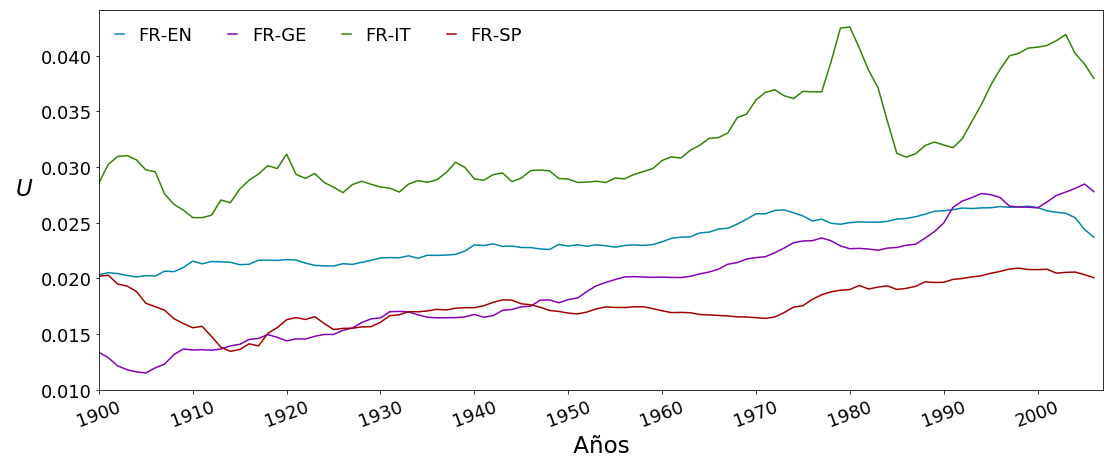
\includegraphics[scale=.36]{UO_FR.png}
	\caption{El francés en los demás idiomas. El italiano empleó más al francés durante todo el siglo XX, caracterizado por palabras comunes en la industria vitivinícola.}
	\label{fig.UO_FR}
\end{figure}


El italiano es el idioma que más utilizó al francés,  la industria vitivinícola, surge como un conector entre ambas lenguas al ser una actividad común en Francia e Italia, con términos como \textit{raisins}, \textit{vin}, \textit{vignoble} y \textit{recolte}.

Los préstamos hacia los demás idiomas son de carácter religioso o político, a pesar de que la búsqueda es en el siglo XX, las mayores migraciones del francés se lograron después de la revolución francesa, entre las palabras que se mantuvieron desde este acontecimiento están  \textit{saint}, \textit{eglise}, \textit{dime}, \textit{reine}, \textit{forteresse}, \textit{napoleon}, \textit{guerre}, \textit{imperiale}, \textit{bastille}, \textit{royals} o \textit{bourgeois}.  


\begin{figure}[h!]
	\centering
	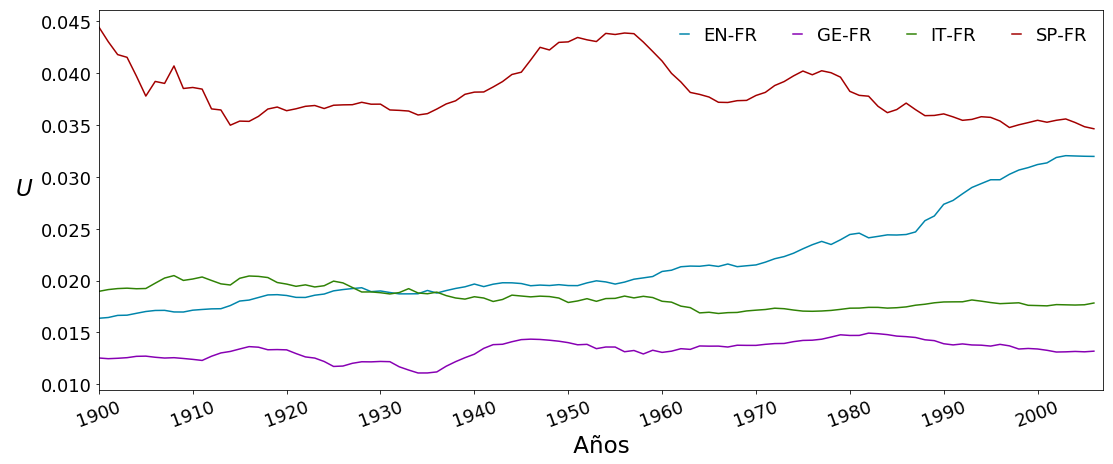
\includegraphics[scale=.36]{UR_FR.png}
	\caption{Los demás idiomas en el francés. El español ha resultado el de mayor presencia en el francés, en su mayoria son palabras con etimologías grecolatinas, comunes para ambas lenguas al provenir de la misma familia lingüística.}
	\label{fig.UR_FR}
\end{figure}
		
Para los prestamos usados en el francés, el español y el inglés se mostraron como los idiomas con mayor presencia, donde el español fue el más utilizado durante todo el siglo, mientras que el inglés resultó el de mayor crecimiento después de 1950. La característica común de los vocablos de ambos idiomas, son palabras con etimología grecolatina,  \textit{depression}, \textit{canal}, \textit{proceso}, \textit{services}, \textit{justice} entre otras. 



\subsection{Alemán} % {{{

\begin{figure}[h!]
	\centering
	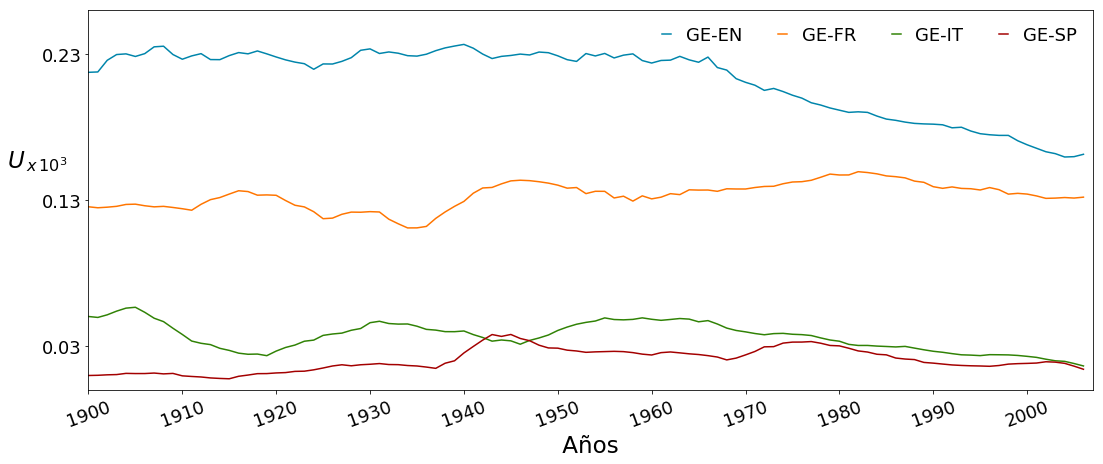
\includegraphics[scale=.36]{UO_GE.png}
	\caption{El alemán en los demás idiomas. La familiaridad de las lenguas germánicas hace posible que el inglés sea el idioma  donde los préstamos del alemán sean continuamente utilizados. Entre las lenguas romances sólo en el francés su uso ha sido constante, mientras que en italiano y español existen periodos donde el empleo del alemán es casi nulo.}
	\label{fig.UO_GE}

\end{figure}

La característica principal de los términos en alemán son personajes germano-parlantes que sobresalieron en algún ámbito, \textit{Hitler}, \textit{Marx}, \textit{Einstein}, \textit{Freud}, \textit{Engels}, \textit{Heidegger}, \textit{Mozart}, \textit{Hegel} y \textit{Nietzsche}; todos ellos fueron préstamos nuevos en el slglo XX. 


\begin{figure}[h!]
	\centering
	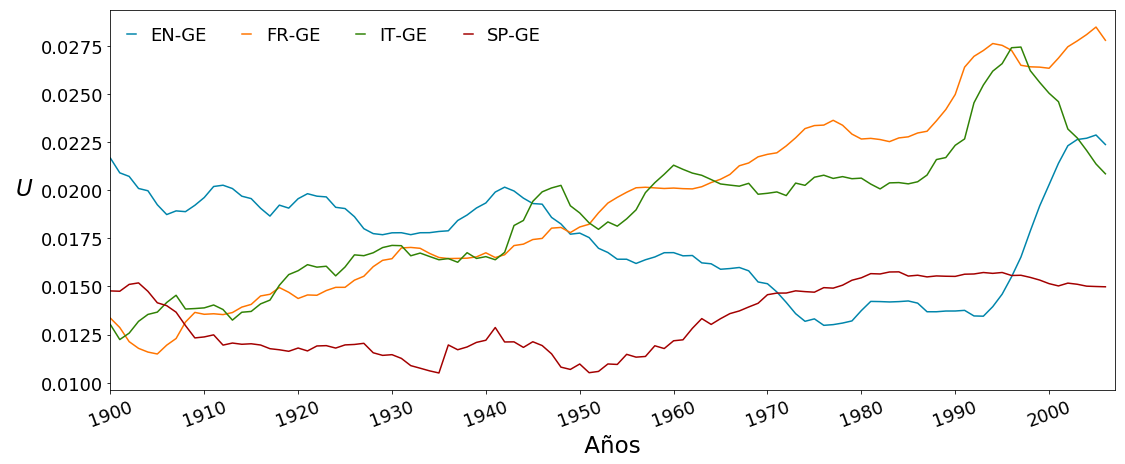
\includegraphics[scale=.36]{UR_GE.png}
	\caption{Los demás idiomas en el alemán. Cada lengua ha tenido un periodo de crecimiento posterior a 1950 tras finalizar la segunda guerra mundial, acontecimiento que influyó para que los demás idiomas impactaran y perduraran en el alemán.}
	\label{fig.UR_GE}
\end{figure}

Como idioma receptor, el alemán adoptó palabras de diferentes campos, tecnológicos y de desarrollo por parte del inglés,  religiosos  por el francés, bélicos del italiano y médicos por el español. La mayoria de los acumulados también fueron prestamos nuevos del siglo XX. 

Cada idioma presentó un periodo de crecimiento posterior a 1950; desde el contexto histórico, al ser vencida Alemania en la segunda guerra mundial, el idioma tuvo que adaptarse a las tendencias donde los demás destacaban. 



% }}}


\subsection{Italiano} % {{{

\begin{figure}[h!]
	\centering
	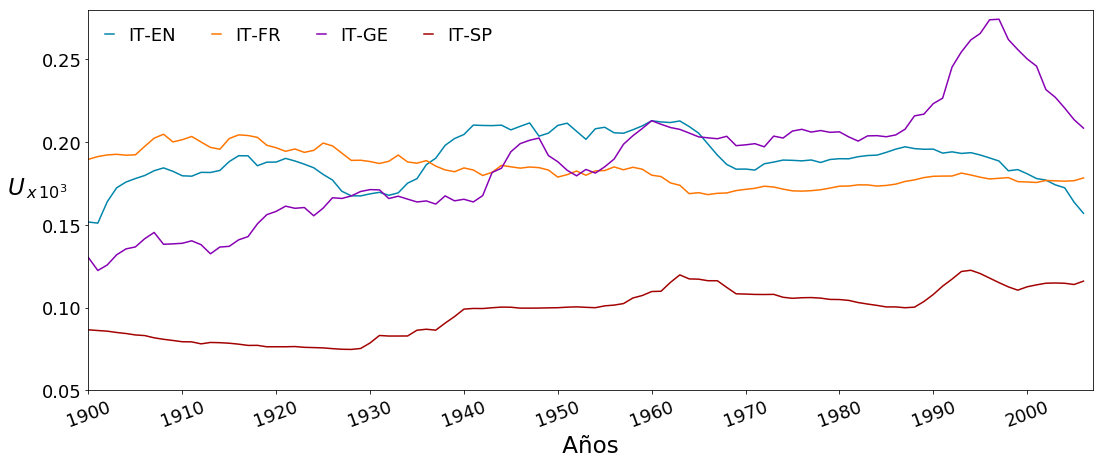
\includegraphics[scale=.36]{UO_IT.png}
	\caption{El italiano en los demás idiomas. A pesar de ser fonéticamente similares y ser tambien una lengua romance,  el español persiste en ser el idioma con menor uso de italiano.}
	\label{fig.UO_IT}
\end{figure}
		
		
El uso del italiano, una única palabra apareció constantemente en los demás idiomas, \textit{mussolini}, posiblemente el personaje más relevante en el siglo pasado, cuya lengua es el italiano.  

Salvo por Mussolini, los demás prestamos italianos no se lograron asociar a un único campo, sin embargo esto muestra la diversidad de temas en los cuales el italiano fue relevante, como la política \textit{sociale}, \textit{liberale}; la religión \textit{santo}, \textit{suora}, \textit{cattedrale}; y la guerra \textit{battaglia}, \textit{regime}.


\begin{figure}[h!]
	\centering
	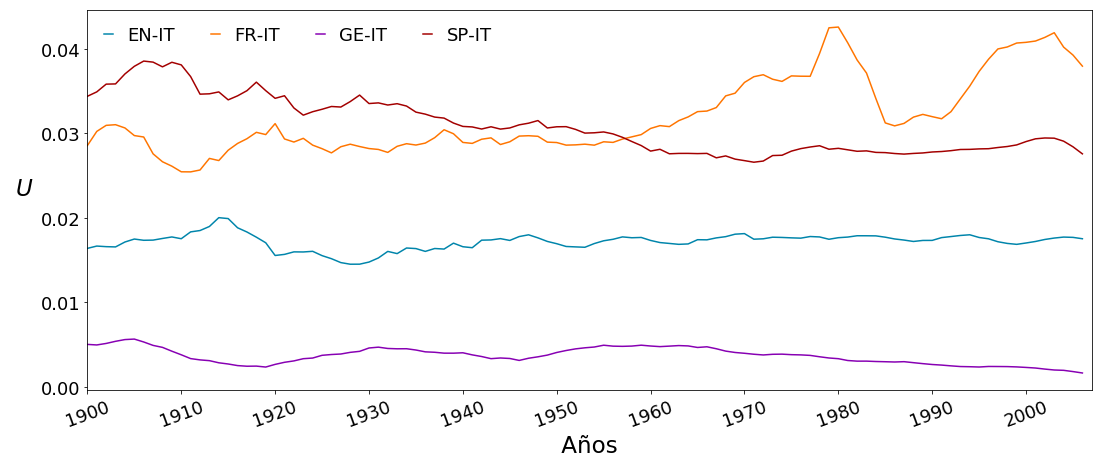
\includegraphics[scale=.36]{UR_IT.png}
	\label{fig.ST_b_IT}
	\caption{Los demás idiomas en el italiano. La proximidad geográfica  entre italia con países cuya lengua es el francés y el alemán ayudó a incrementar el uso de estos en el italiano. A pesar de que el inglés se difundió como un idioma universal para la comunicación, su uso en el italiano no ha mostrado un incremento en todo el siglo XX. }
	\label{fig.UR_IT}
\end{figure}

El contenido de las palabras que tomó el italiano, es igualmente variado, por parte del ingles son conceptos de la tecnología, por el francés a la industria vitivinícola, con el alemán a personajes relevantes de esta lengua, y del español a nombres de países o ciudades hispanohablantes \textit{México}, \textit{Chile}, \textit{Argentina}, \textit{Montevideo} o \textit{Peru}. 

% }}}


\subsection{Español} % {{{

\begin{figure}[h!] % {{{
	\centering
	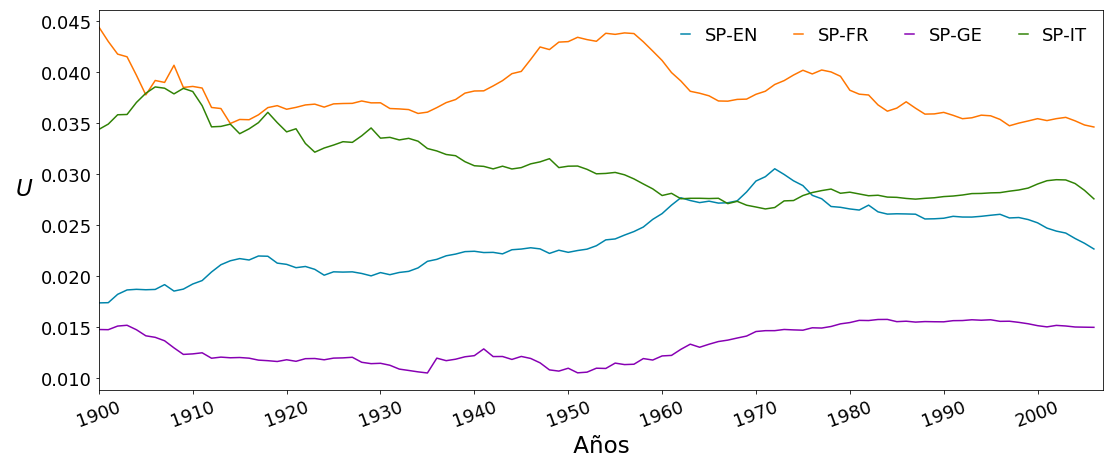
\includegraphics[scale=.36]{UO_SP.png}
	\caption{El español en los demás idiomas. Los idiomas que más emplean español son aquellos con los que comparte una relación etimológica, francés e italiano por ser lenguas romances y con el ingles al tener este idioma una base de palabras grecolatinas.  Los préstamos destacan al ser términos médicos y nombres de países y ciudades hispanohablantes.}
	\label{fig.UO_SP}
	
\end{figure}

Entre los diferentes receptores, el francés fue el idioma que más empleo al español, seguido del italiano y del inglés; estas tres lenguas son las las que más relación etimológica tienen con el español.  

Entre los gráficos de la sección \ref{palabras.acumuladas.apendice}, se observo que el uso del español en los demás idiomas, es mayor que el uso de los otros en él, sin importar la combinacion que se trate.

Nuevamente,  el ámbito medico caracterizó a las palabras más empleadas con origen español, entre ellas \textit{terapia}, \textit{lepra}, \textit{tumor}, \textit{syphilis}, \textit{virus} o \textit{renal}. 

		
\begin{figure}[h!] % {{{
	\centering
	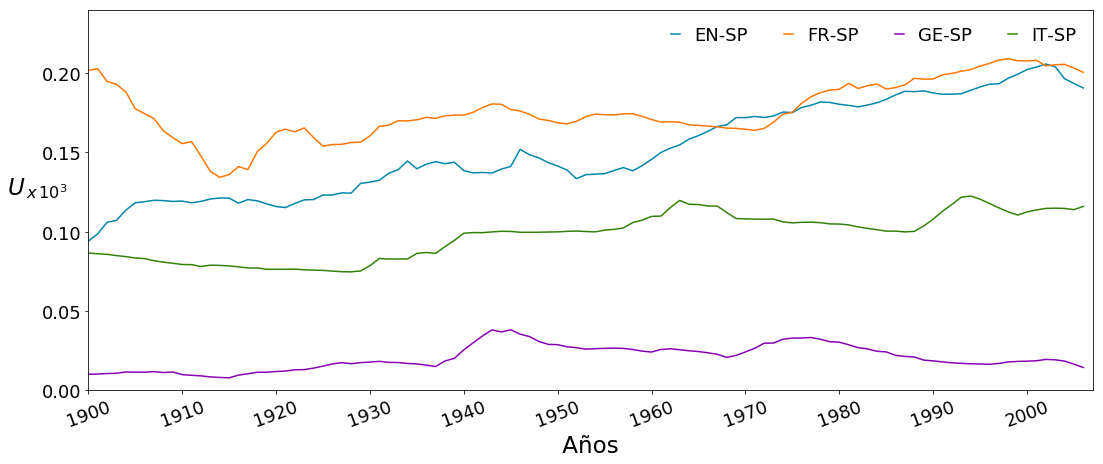
\includegraphics[scale=.36]{UR_SP.png}
	\label{fig.ST_b_SP}
	\caption{Los demás idiomas en el español. Inglés y francés son los idiomas que mayor uso han tenido en el español, llegando a ser equiparables en los últimos cuarenta años. El alemán ha sido el que menos ha impactado, siendo su mayor crecimiento  alrededor de 1940.}
	\label{fig.UR_SP}
\end{figure}


En las discusiones anteriores, se ha mencionado el tipo de palabras que los idiomas aportan al español, del ingles los préstamos son de carácter tecnológico y del desarrollo industrial, del alemán son apellidos de personajes destacados en un campo especifico, mientras que del francés y el italiano son tipo religioso, histórico y político. 






% }}}
% }}}
\section{Comentarios y complementos del método} % {{{


El determinar la influencia entre idiomas a través del uso, ha mostrado que el idioma que más cantidad de palabras tiene en otro no siempre es el más utilizado, el mayor uso se da en aquel cuyos préstamos tengan menores rangos. 

Por el momento sólo es posible describir que originó las variaciones en el uso o en la cantidad de palabras nuevas, no es posible predecir como se comportaran los idiomas en el futuro. Se destaca a los eventos como una característica que  hace fluir a las palabras, al modificar el uso de un idioma en otro tras el suceso. 


Una mejor información de como los eventos alteran a los idiomas se podría extraer si se comparará el uso con con  datos de los países de alguna habla como lo pueden ser  el crecimiento economizo, el producto interno bruto, la alfabetización, la mortalidad, las migraciones de personas, entre otros. 

%Una mejor información de como los eventos alteran a los idiomas se podría extraer si se compararán las características de los prestamos con  datos de los países de alguna habla como lo pueden ser  el crecimiento economizo, el producto interno bruto, la alfabetización, la mortalidad, las migraciones de personas, entre otros.

%En todo el siglo XX y la primer década del XXI, el inglés y el alemán han sido los idiomas más cambiantes en los papeles de origen y receptor. En cualquier combinación con otro idioma el uso ha sido alterado en alguna época. 
%El inglés al ser el que más creció en tres idiomas (francés, alemán y español), complementando los resultados del capitulo anterior, al ser el idioma que más palabras nuevas exportó.  El alemán como el receptor donde los diferentes orígenes aumentaron su usó tras la segunda guerra mundial; el uso ha sido semejante a los préstamos nuevos, ha sido el receptor que más recibió. 
%Ambos análisis se complementan,  el idioma más influyente ha aportado más palabras nuevas y aquellas que se van acumulando resultan las de mayor incremento en el uso. El idioma más influenciado recibió la mayor cantidad de palabras nuevas y el uso que han tenido los demás ha sido también el del mayor incremento. 

 




% }}}

